\documentclass[10pt]{article}
\usepackage[margin=1.0cm]{geometry}
\usepackage[T1]{fontenc}
\usepackage{lmodern}
\usepackage{xcolor}
\usepackage{tikz}
\usepackage{pgfplots}
\usepgfplotslibrary{statistics}
\pgfplotsset{compat=1.18}
\definecolor{srblue}{HTML}{2F6B9A}
\definecolor{opencvorange}{HTML}{D97706}
\definecolor{fps2blue}{HTML}{B9D7EA}
\definecolor{fps5orange}{HTML}{F6C28B}
\definecolor{stslightgreen}{HTML}{A7D8B1}
\definecolor{stsstronggreen}{HTML}{208B3A}
\definecolor{sugarlightpurple}{HTML}{CBB7E8}
\definecolor{sugarstrongpurple}{HTML}{763A9B}
\definecolor{stsedge}{HTML}{1D4E89}
\definecolor{sugaredge}{HTML}{B45309}
\definecolor{incompletegray}{HTML}{9CA3AF}
\definecolor{deltared}{HTML}{B91C1C}
\definecolor{deltagreen}{HTML}{15803D}
\begin{document}
\pagestyle{empty}
\begin{center}
{\Large\bfseries SuGaR-Coarse minus STS: Mittelwerte}\\[3pt]
{\small Gepaarte Differenz der gemittelten Renderingmetriken}\\[8pt]
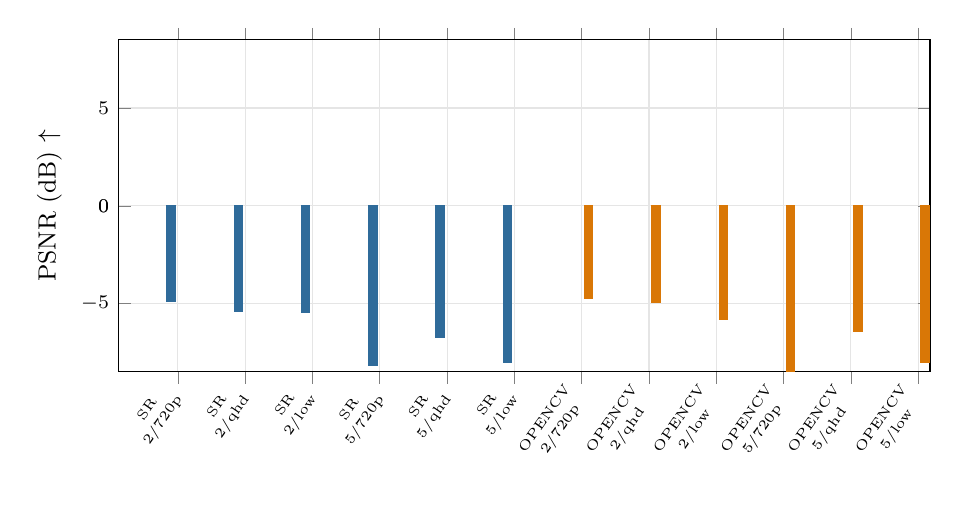
\begin{tikzpicture}
\begin{axis}[height=5.8cm,width=0.98\linewidth,ybar,bar width=2.8pt,enlarge x limits=0.015,xmin=-0.7,ymin=-8.49,ymax=8.49,xtick=data,xticklabels={{\shortstack{SR\\2/720p}},{\shortstack{SR\\2/qhd}},{\shortstack{SR\\2/low}},{\shortstack{SR\\5/720p}},{\shortstack{SR\\5/qhd}},{\shortstack{SR\\5/low}},{\shortstack{OPENCV\\2/720p}},{\shortstack{OPENCV\\2/qhd}},{\shortstack{OPENCV\\2/low}},{\shortstack{OPENCV\\5/720p}},{\shortstack{OPENCV\\5/qhd}},{\shortstack{OPENCV\\5/low}}},x tick label style={font=\tiny,rotate=55,anchor=east},ylabel style={font=\small},tick label style={font=\scriptsize},ylabel={PSNR (dB) $\uparrow$},grid=major,grid style={gray!20},legend style={font=\scriptsize,at={(1.0,1.15)},anchor=south east,draw=none,fill=white,fill opacity=0.9,text opacity=1},xtick={0,1,2,3,4,5,6,7,8,9,10,11},ymin=-8.49,ymax=8.49,extra y ticks={0},extra y tick style={grid=major,black}]
\addplot+[ybar,bar width=3pt,fill=srblue,draw=srblue] coordinates {(0,-4.87724743) (1,-5.38735604) (2,-5.42780189) (3,-8.17899579) (4,-6.73127323) (5,-8.01510125)};
\addplot+[ybar,bar width=3pt,fill=opencvorange,draw=opencvorange] coordinates {(6,-4.74502493) (7,-4.93752393) (8,-5.79314817) (9,-8.48373744) (10,-6.42777737) (11,-7.98586752)};
\end{axis}
\end{tikzpicture}\par\vspace{2pt}
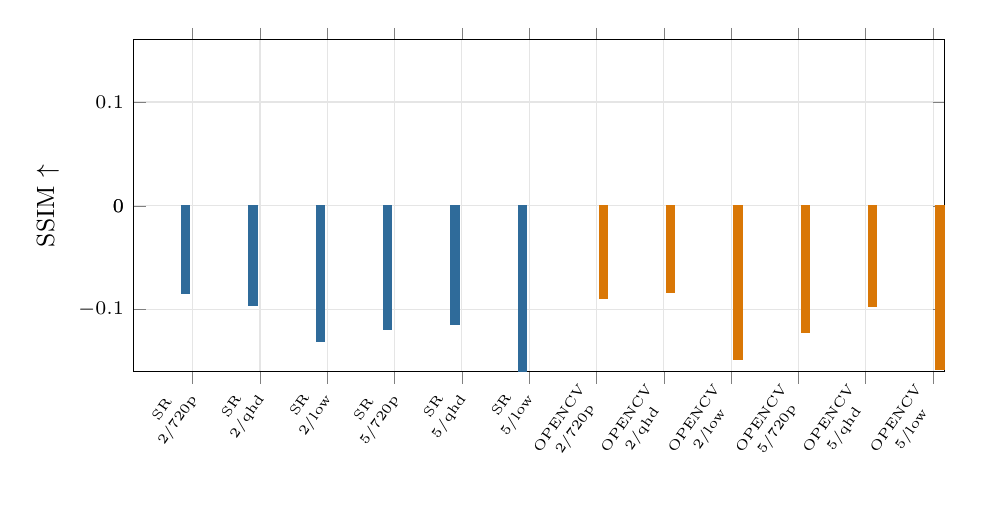
\begin{tikzpicture}
\begin{axis}[height=5.8cm,width=0.98\linewidth,ybar,bar width=2.8pt,enlarge x limits=0.015,xmin=-0.7,ymin=-0.16,ymax=0.16,xtick=data,xticklabels={{\shortstack{SR\\2/720p}},{\shortstack{SR\\2/qhd}},{\shortstack{SR\\2/low}},{\shortstack{SR\\5/720p}},{\shortstack{SR\\5/qhd}},{\shortstack{SR\\5/low}},{\shortstack{OPENCV\\2/720p}},{\shortstack{OPENCV\\2/qhd}},{\shortstack{OPENCV\\2/low}},{\shortstack{OPENCV\\5/720p}},{\shortstack{OPENCV\\5/qhd}},{\shortstack{OPENCV\\5/low}}},x tick label style={font=\tiny,rotate=55,anchor=east},ylabel style={font=\small},tick label style={font=\scriptsize},ylabel={SSIM $\uparrow$},grid=major,grid style={gray!20},legend style={font=\scriptsize,at={(1.0,1.15)},anchor=south east,draw=none,fill=white,fill opacity=0.9,text opacity=1},xtick={0,1,2,3,4,5,6,7,8,9,10,11},ymin=-0.16,ymax=0.16,extra y ticks={0},extra y tick style={grid=major,black}]
\addplot+[ybar,bar width=3pt,fill=srblue,draw=srblue] coordinates {(0,-0.08422103) (1,-0.09574666) (2,-0.13081713) (3,-0.11864725) (4,-0.11474491) (5,-0.15950086)};
\addplot+[ybar,bar width=3pt,fill=opencvorange,draw=opencvorange] coordinates {(6,-0.08882320) (7,-0.08334616) (8,-0.14801196) (9,-0.12228578) (10,-0.09695547) (11,-0.15786545)};
\end{axis}
\end{tikzpicture}\par\vspace{2pt}
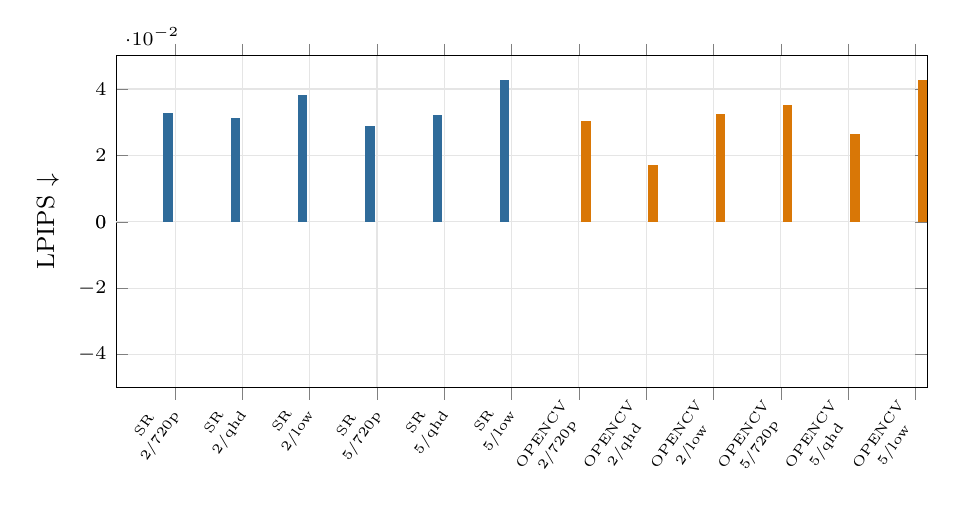
\begin{tikzpicture}
\begin{axis}[height=5.8cm,width=0.98\linewidth,ybar,bar width=2.8pt,enlarge x limits=0.015,xmin=-0.7,ymin=-0.05,ymax=0.05,xtick=data,xticklabels={{\shortstack{SR\\2/720p}},{\shortstack{SR\\2/qhd}},{\shortstack{SR\\2/low}},{\shortstack{SR\\5/720p}},{\shortstack{SR\\5/qhd}},{\shortstack{SR\\5/low}},{\shortstack{OPENCV\\2/720p}},{\shortstack{OPENCV\\2/qhd}},{\shortstack{OPENCV\\2/low}},{\shortstack{OPENCV\\5/720p}},{\shortstack{OPENCV\\5/qhd}},{\shortstack{OPENCV\\5/low}}},x tick label style={font=\tiny,rotate=55,anchor=east},ylabel style={font=\small},tick label style={font=\scriptsize},ylabel={LPIPS $\downarrow$},grid=major,grid style={gray!20},legend style={font=\scriptsize,at={(1.0,1.15)},anchor=south east,draw=none,fill=white,fill opacity=0.9,text opacity=1},xtick={0,1,2,3,4,5,6,7,8,9,10,11},ymin=-0.05,ymax=0.05,extra y ticks={0},extra y tick style={grid=major,black}]
\addplot+[ybar,bar width=3pt,fill=srblue,draw=srblue] coordinates {(0,0.03265356) (1,0.03098150) (2,0.03799666) (3,0.02856731) (4,0.03209947) (5,0.04259803)};
\addplot+[ybar,bar width=3pt,fill=opencvorange,draw=opencvorange] coordinates {(6,0.03008912) (7,0.01706957) (8,0.03237062) (9,0.03494588) (10,0.02637594) (11,0.04255807)};
\end{axis}
\end{tikzpicture}\par\vspace{2pt}
\vspace{3pt}
\begin{minipage}{0.98\linewidth}\scriptsize Delta = SuGaR-Coarse minus STS for the same follow-up run. The x-label explicitly contains SR or OPENCV, FPS and resolution. For LPIPS, a negative delta favours SuGaR-Coarse because lower LPIPS is better. The paired comparison is only a rendering-stage comparison, not a mesh-accuracy test.\end{minipage}
\end{center}
\end{document}